% !TeX program = pdflatex
\documentclass[border=6pt]{standalone}
\usepackage{tikz}
\usetikzlibrary{arrows.meta, positioning, fit, backgrounds}

\definecolor{MediumRed}{rgb}{0.925, 0.345, 0.345}
\definecolor{MediumGreen}{rgb}{0.37, 0.7, 0.66}
\definecolor{MediumBlue}{rgb}{0.015, 0.315, 0.45}
\definecolor{DarkBlue}{rgb}{0.05, 0.15, 0.35}

\begin{document}
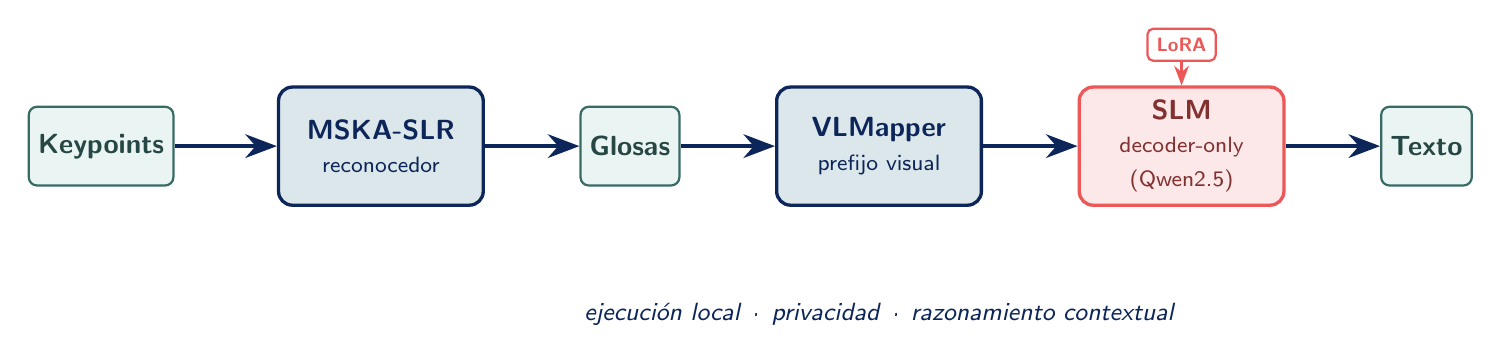
\begin{tikzpicture}[
    font=\sffamily,
    stage/.style={draw=DarkBlue, very thick, rounded corners=5pt,
        fill=MediumBlue!14, align=center, text=DarkBlue,
        minimum width=2.6cm, minimum height=1.5cm},
    data/.style={draw=MediumGreen!60!black, thick, rounded corners=3pt,
        fill=MediumGreen!14, align=center, text=MediumGreen!40!black,
        minimum height=1.0cm},
    flow/.style={-{Stealth[length=4mm]}, line width=1.4pt, DarkBlue},
]

% entrada
\node[data] (kp) {\textbf{Keypoints}};

% MSKA-SLR
\node[stage, right=1.3cm of kp] (mska) {\textbf{MSKA-SLR}\\\footnotesize reconocedor};

% glosas
\node[data, right=1.2cm of mska] (gloss) {\textbf{Glosas}};

% VLMapper
\node[stage, right=1.2cm of gloss] (vlm) {\textbf{VLMapper}\\\footnotesize prefijo visual};

% SLM
\node[stage, right=1.2cm of vlm, fill=MediumRed!14, draw=MediumRed,
      text=MediumRed!55!black] (slm)
    {\textbf{SLM}\\\footnotesize decoder-only\\\footnotesize (Qwen2.5)};

% salida
\node[data, right=1.2cm of slm] (txt) {\textbf{Texto}};

\foreach \a/\b in {kp/mska, mska/gloss, gloss/vlm, vlm/slm, slm/txt}
    \draw[flow] (\a) -- (\b);

% badge LoRA sobre el SLM
\node[draw=MediumRed, thick, rounded corners=2pt, fill=white,
      text=MediumRed, font=\sffamily\scriptsize\bfseries, above=3mm of slm] (lora)
    {LoRA};
\draw[-{Stealth[length=2.5mm]}, MediumRed, thick] (lora) -- (slm);

% pie
\node[font=\sffamily\small\itshape, text=DarkBlue, below=1.1cm of vlm]
    {ejecución local\, ·\, privacidad\, ·\, razonamiento contextual};

\end{tikzpicture}
\end{document}
